\documentclass[12pt,a4paper,titlepage,listof=totoc,bibliography=totoc,chapteratlists=0pt]{scrreprt}

\begin{filecontents*}{\jobname.xmpdata}
	\Keywords{VR, IOT, TODO}
	\Title{Pool-Überwachung}
	\Author{Florian Wilflingseder}
\end{filecontents*}

\setcounter{tocdepth}{1}

\usepackage[utf8]{inputenc}
\usepackage[T1]{fontenc}
\usepackage{amsmath}
\usepackage{amsfonts}
\usepackage{amssymb}
\usepackage[table]{xcolor}
\usepackage{graphicx}
\usepackage[left=3.50cm, right=2.00cm, top=2.00cm, bottom=2.00cm,foot=1cm]{geometry}
\usepackage[splitrule,hang,flushmargin,multiple,bottom]{footmisc}
\usepackage{lmodern, textcomp}
\usepackage{lmodern}
\usepackage{pdfpages}
\usepackage[ngerman]{babel}
\usepackage{multicol}
\usepackage{float}
\usepackage{array,tabularx,booktabs}
\usepackage{ragged2e}
\usepackage{lipsum}
\usepackage{wrapfig}

\newcolumntype{M}[1]{>{\centering\arraybackslash}m{#1}}

\usepackage{enumitem}
\newlist{compactitem}{itemize}{3}
\setlist[compactitem,1]{label=\textbullet, nosep,leftmargin=1.5em,labelwidth=*,align=left}
\setlist[compactitem,2]{label=--, nosep,leftmargin=1.5em,labelwidth=*,align=left}
\setlist[compactitem,3]{label=\textopenbullet, nosep,leftmargin=1.5em,labelwidth=*,align=left}
\newlist{compactenum}{enumerate}{3}
\setlist[compactenum,1]{label=\arabic*., nosep,leftmargin=1.5em,labelwidth=*,align=left}
\setlist[compactenum,2]{label=\alph*., nosep,leftmargin=1.5em,labelwidth=*,align=left}
\setlist[compactenum,3]{label=\roman*., nosep,leftmargin=1.5em,labelwidth=*,align=left}
\newlist{compactdesc}{description}{3}
\setlist[compactdesc]{leftmargin=1.5em,labelwidth=*,align=left}

\usepackage{microtype}

\usepackage[parfill]{parskip}

\definecolor{bluekeywords}{rgb}{0.13,0.13,1}
\definecolor{greencomments}{rgb}{0,0.5,0}
\definecolor{redstrings}{rgb}{0.9,0,0}
\definecolor{lightgray}{gray}{0.9}
\definecolor{lightblue}{rgb}{0.93,0.95,1.0}

\usepackage{listings}

\makeatletter
\lstdefinestyle{lststyle}{
	basicstyle=%
	\ttfamily
	\lst@ifdisplaystyle\scriptsize\fi
}
\makeatother

\renewcommand{\lstlistlistingname}{List of Listings}
% TODO: define other languages as needed
\lstset{language=Python,
numbers=left,               
numberstyle=\tiny,          
showspaces=false,
showtabs=false,
breaklines=true,
lineskip=-1pt,
tabsize=2,
showstringspaces=false,
breakatwhitespace=true,
escapeinside={(*@}{@*)},
commentstyle=\color{greencomments},
keywordstyle=\color{bluekeywords}\bfseries,
stringstyle=\color{redstrings},
style=lststyle,
xleftmargin=17pt,
         framexleftmargin=17pt,
         framexrightmargin=5pt,
         framexbottommargin=4pt
}
\lstset{
morekeywords={base,var,in,out,dynamic,from,where,select,orderby,function,\$,group,by,into,yield,async,await,@,None,self,as,elif,with}
}
\lstdefinelanguage{TypeScript}{
	keywords={typeof, new, true, false, catch, function, return, null, switch, var, if, in, while, do, else, case, break, void, number, string, boolean, module, \$, export, for, this},
	keywordstyle=\color{blue}\bfseries,
	ndkeywords={class, export, boolean, throw, implements, import, this},
	ndkeywordstyle=\color{darkgray}\bfseries,
	identifierstyle=\color{black},
	sensitive=false,
	comment=[l]{//},
	morecomment=[s]{/*}{*/},
	commentstyle=\color{purple}\ttfamily,
	stringstyle=\color{red}\ttfamily,
	morestring=[b]',
	morestring=[b]"
}
\usepackage{caption}
\DeclareCaptionFont{white}{\color{white}}
\DeclareCaptionFormat{listing}{\colorbox[cmyk]{0.43, 0.35, 0.35,0.01}{\parbox{\textwidth}{\hspace{10pt}#1#2#3}}}
\captionsetup[lstlisting]{format=listing,labelfont=white,textfont=white} 
\captionsetup[table]{justification=centering, singlelinecheck=false}

\usepackage{subcaption}

\usepackage{setspace}
\newcommand{\MSonehalfspacing}{%
	\setstretch{1.44}%  default
	\ifcase \@ptsize \relax % 10pt
	\setstretch {1.448}%
	\or % 11pt
	\setstretch {1.399}%
	\or % 12pt
	\setstretch {1.433}%
	\fi
}

\newcommand{\setauthor}[1]{\ohead[]{#1}}

\usepackage[automark]{scrlayer-scrpage}
\pagestyle{scrheadings}
\automark{chapter}
\renewcommand\sectionmark[1]{\markright{\MakeMarkcase {\thesection\hskip .5em\relax#1}}}
\rohead{\ifnum\expandafter\pdfstrcmp\botmark=0 \rightmark\else\leftmark{} --- \rightmark\fi}
\ihead[]{\headmark}
\chead[]{}
\ohead{}
\cfoot[]{}
\ofoot[\pagemark]{\pagemark}
\setheadsepline{.1pt}

\usepackage[hyphens]{url}

\usepackage[a-1b]{pdfx}

\usepackage{hyperref}
\hypersetup{pdfa}

\usepackage[nonumberlist,toc,nopostdot]{glossaries}

\usepackage{chngcntr}
\counterwithout{footnote}{chapter}
\counterwithout{figure}{chapter}
\counterwithout{table}{chapter}
\AtBeginDocument{
	\counterwithout{lstlisting}{chapter}
	\urlstyle{sf}
}
\newcounter{RPages}

\makeatletter
\def\bstctlcite{\@ifnextchar[{\@bstctlcite}{\@bstctlcite[@auxout]}}
\def\@bstctlcite[#1]#2{\@bsphack
	\@for\@citeb:=#2\do{%
		\edef\@citeb{\expandafter\@firstofone\@citeb}%
		\if@filesw\immediate\write\csname #1\endcsname{\string\citation{\@citeb}}\fi}%
	\@esphack}
\makeatother

\clubpenalty=10000
\widowpenalty=10000
\displaywidowpenalty=10000
\interfootnotelinepenalty=10000

\title{SPA TemperaturSensor}
\author{Florian Wilflingseder}

\makeindex
\makeglossaries
\begin{document}
\bstctlcite{IEEEexample:BSTcontrol}
\newcommand{\reminder}[1]
{ \textcolor{red}{<[{\bf\marginpar{\mbox{$<==$}} #1 }]>} }
\newcommand{\icode}[1]{\lstinline$#1$}
%\urlstyle{same}
%\setstretch{1.5}
\setstretch {1.433}
\renewcommand{\arraystretch}{1.2}

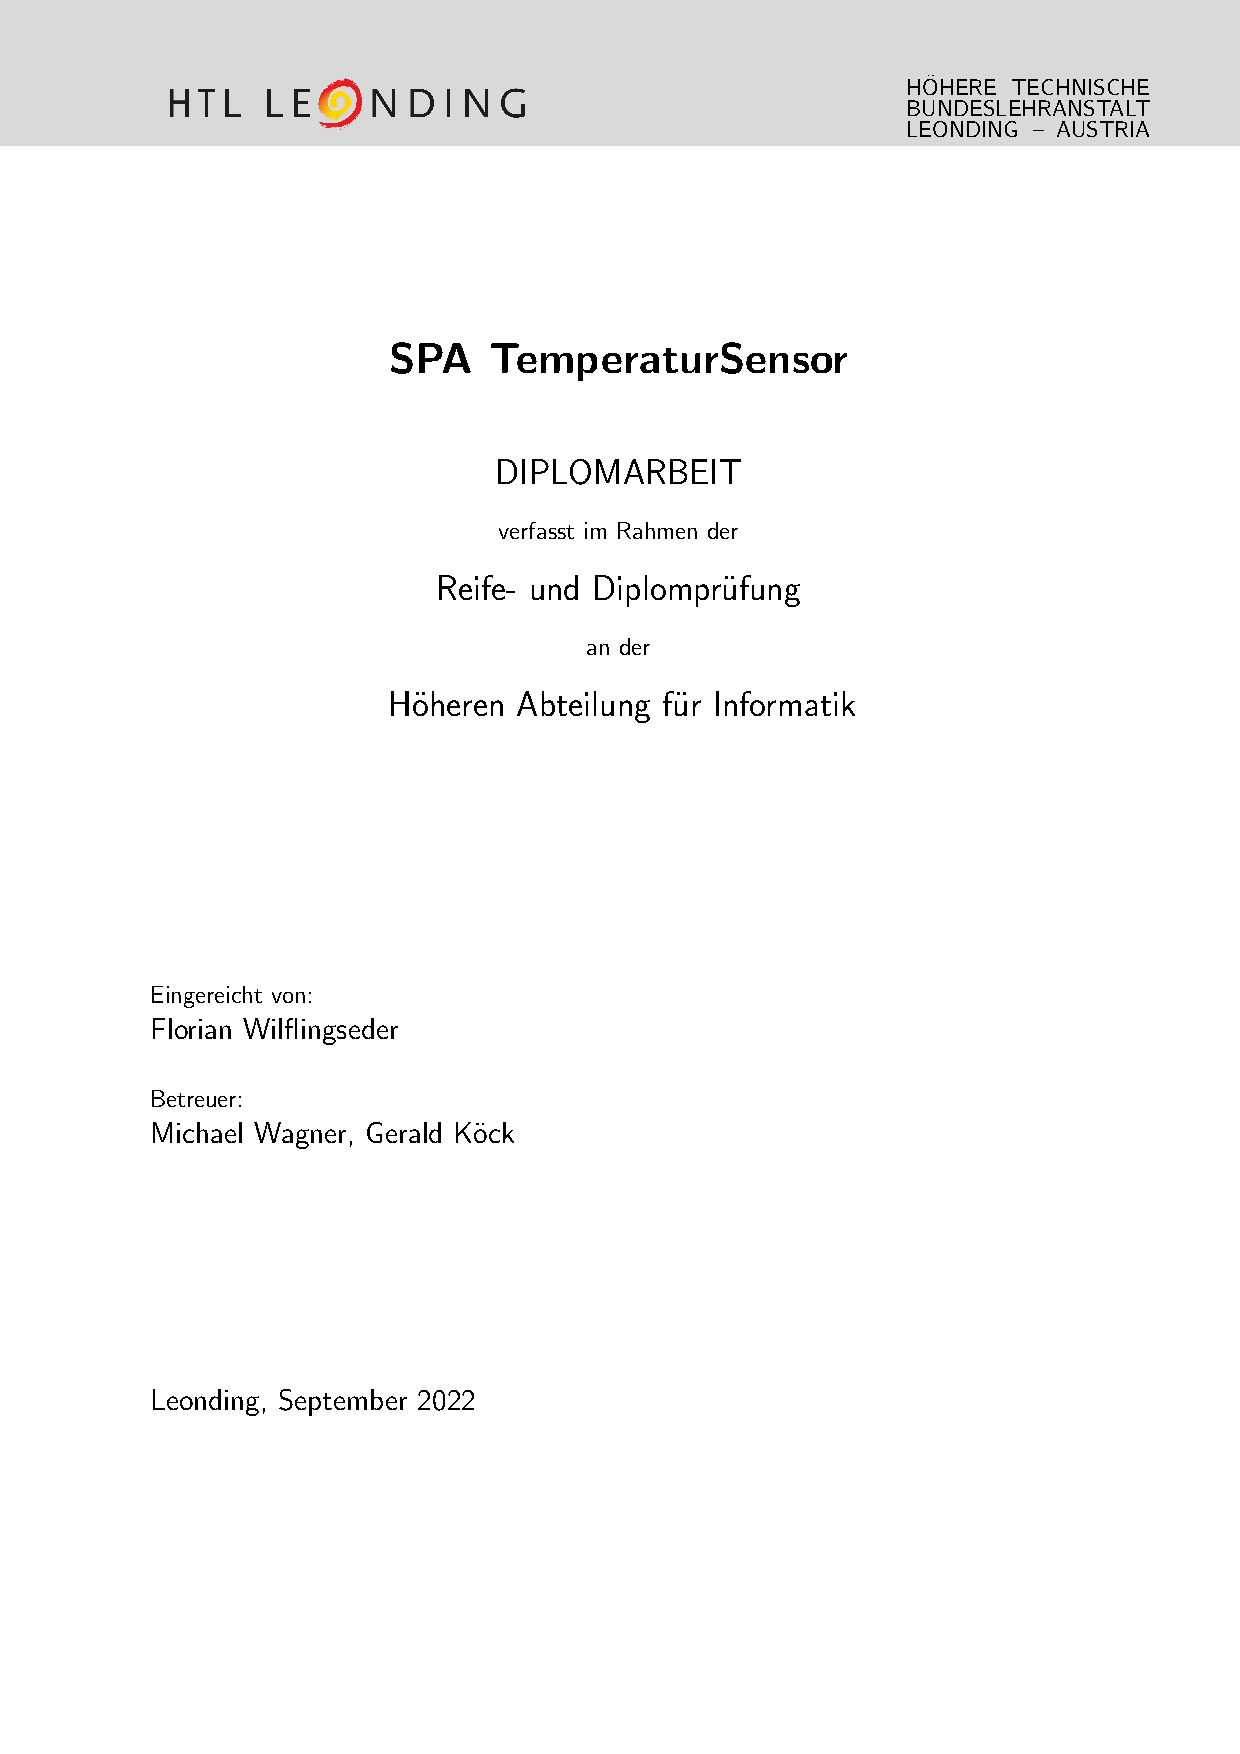
\includepdf{./titlepage/coversheet}
\pagenumbering{Roman}
\newpage


\pagestyle{plain}

\renewcommand{\lstlistlistingname}{Quellcodeverzeichnis}

\tableofcontents
\newpage
\setcounter{RPages}{\value{page}}
\setcounter{page}{0}
\pagenumbering{arabic}
\pagestyle{scrheadings}


\begin{spacing}{1}
\chapter{Marktanalyse}
\end{spacing}

\section{Markt:}
Das Produkt richtet sich an Privatpersonen 
die einen Garten mit einer beliebigen Schwimmanlage besitzen. 
Die Altersgruppe wird sich an alle Geschlechter zwischen 25-60 Jahren richten. 
Das Produkt wird besonders attraktiv für Erwachsene 
mit Kindern sein die noch Beaufsichtigung benötigen wenn sie sich
in der Nähe von Gewässern aufhalten, wegen der Wellenerkennungsfunktion.
\section{Mitbewerber:}
\textbf{Smart Poolthermometer Starter Set:}


Das Set besteht aus 3 Teilen, einem schwimmenden Poolthermometer, 
einem Aussenfühler und einem Netzwerk Gateway. Kommt mit einer eigenen Smart App dazu. 
Es kann die Wassertemperatur die Luftaußentemperatur und die Luftfeuchtigkeit gemessen werden.
Netzwerkfähig (funkt das Gateway (bei freier Sichtline bis zu 100 Meter) an, 
der mit dem W-Lan Verbunden ist). Unterstützt Amazon Alexa und Conrad Connect. 
Wie der Pool so auch der Außenthermometer werden mit 2x AA Batterien betrieben. 
Der Außenthermometer ist dazu nicht Wetterfest und es muss eine extra Schutzhülle 
mitbestellt werden. Details über die einzelnen Bauteile werden nicht bekannt gegeben.


\textbf{WLAN Swimming Pool Thermometer Bundle|Inkbird:}


Hat ein Aufstellbaren-Display, Outdoor Hygrometer und Thermometer, 
Datenlogger, Export-Funktion, Cloud, App. 
Es kann die Wassertemperatur die Luftaußentemperatur und die Luftfeuchtigkeit gemessen werden.
Es wird nur ein Display zur Anzeige mitgeliefert und man 
kann seine Daten 12 Monate kostenlos in einer Cloud speichern.
Details über die einzelnen Bauteile werden nicht bekannt gegeben.

\newpage
\textbf{Elektrobock ELBO-073 Wireless Pool Alarm:}


Dieses Gerät dient nur als Alarmanlage für das Wasser. 
Es erkennt den Wellengang und löst seine eingebaute Sirene aus. 
Das Gerät besitz ein Gegenstück welchen man in seiner Nähe an einer Steckdose anstecken 
kann und ein Signal von dem Sender im Wasser bekommt. 
Dadurch läutet die Sirene an 2 Standorten. Ansonsten bietet dieses keine zusätzlichen Funktionen.
Details über die einzelnen Bauteile werden nicht bekannt gegeben.



\begin{spacing}{1}
\chapter{Technologien}
\end{spacing}


\section{ESP32:}


\textbf{}
\begin{itemize}
    \item Der ESP32 unterstützt bis zu 4 × 16 MB externen Speicher.
    \item Man kann den internen Takt (8 MHz) oder einen
    externen Quarztakt mit üblicherweise 160 MHz nutzen. 
    Wenn man den Prozessor zurück setzt übernimmt er auch das System-Timing.
    \item Hall-Sensor: Kann für die Messung von Magnetfeldschwankungen genutzt werden.
    \item Ein interner Temperatursensor mit einem Messbereich von –40 bis 125 Grad ist ebenfalls vorhanden.
    Die analogen Messwerte werden wie bei dem Hall-Sensor
    von einem Analog-Digital-Wandler digitalisiert. 
    In neueren Modellen ist kein Temperatur Sensor mehr verbaut.
    \item Es sind 34 GPIOs (universelle Ein- und Ausgänge) vorhanden. 
    Verwendet werden diese für Ein-und Ausgabe analoger und digitaler Signale. 
    Die Pins sind mehrfach belegt. 
    Mit internen Pull-down und Pull-up-Widerständen können definierte Zustände herbeigeführt werden.
    \item Der ESP32 kann Signale von bis zu zehn unterschiedlichen TouchSensoren verarbeiten. 
    \item Der ESP32 Unterstützt Bluetooth als auch W-Lan im 2.4-GHz Bereich und kann diese 
    Empfangen und Senden. 
    \item Das WLAN hat einen IEE 802.11 Standard.
    \item Es wird Bluetooth 4.2 und Bluetooth low-energy unterstützt.
    \item UART (Universal Asynchronous Receiver Transmitter) 
    \item Impulse können mit acht Impulszählern erfasst werden. 
    \item Der ESP32 hat vier 64-Bit-Universaltimer. Diese kann man via Software steuern.
    \item Es gibt Watchdog-Timer. Man unterscheidet zwischen Main-Watchdog-Timern und RTC-Watchdog-Timern. 
    Auslösen kann man hiermit einen CPU-Reset , ein Core-Reset oder ein Interrupt.
    \item  12-Bit-A/D-Wandler (Analog-Digital-Wandler) mit 18 Kanälen 
    \item  8-Bit-DAC (Digital-Analog-Wandler)
    \item SPI-Schnittstellen (SPI1, HSPI and VSPI) mit Master- oder Slave-Modus
    \item Es werden zwei I2C-Bus-Schnittstellen vorgehalten, die im Master- oder SlaveModus betrieben werden können.
    \item Pulsweitenmodulation (PWM) um Geräte wie Motoren, elektrische Heizungen oder Ähnliches zu steuern. 
    \item Ein Infrarot-Controller, mit 8 programmierbaren Kanälen.
    
\end{itemize}


\newpage

\pagenumbering{Roman}
\setcounter{page}{\value{RPages}}
%\setlength{\glsdescwidth}{0.8\linewidth}
\glsnogroupskiptrue
\printglossary[title=Glossar,toctitle=Glossar] %,style=long]
\spacing{1}{
%\bibliographystyle{IEEEtran}
\bibliographystyle{ieeetrande}
\bibliography{bib}
}
\listoffigures
\listoftables
\lstlistoflistings
\appendix
\addchap{Anhang}
\end{document}

